\documentclass{VUMIFPSbakalaurinis}
\usepackage{algorithmicx}
\usepackage{algorithm}
\usepackage{algpseudocode}
\usepackage{amsfonts}
\usepackage{amsmath}
\usepackage{bm}
\usepackage{caption}
\usepackage{color}
\usepackage{float}
\usepackage{graphicx}
\usepackage{listings}
\usepackage{subfig}
\usepackage{wrapfig}

\usepackage{enumitem}
\setitemize{noitemsep,topsep=0pt,parsep=0pt,partopsep=0pt}
\setenumerate{noitemsep,topsep=0pt,parsep=0pt,partopsep=0pt}

\hbadness=100000
% Titulinio aprašas
\university{Vilniaus universitetas}
\faculty{Matematikos ir informatikos fakultetas}
\department{Programų sistemų studijų programa}
\papertype{Mokslo tiriamasis darbas II}
\title{Srautinio apdorojimo sistemų balansavimas taikant mašininį mokymąsi}
\titleineng{Balancing stream processing systems using machine learning}
\author{Vytautas Žilinas}
\supervisor{Partn. doc. Andrius Adamonis}
\reviewer{Prof. dr. Aistis Raudys}
\date{Vilnius – \the\year}

% Nustatymai
% \setmainfont{Palemonas}   % Pakeisti teksto šriftą į Palemonas (turi būti įdiegtas sistemoje)
\bibliography{bibliografija}

\begin{document} 
\maketitle

\cleardoublepage\pagenumbering{arabic}
\setcounter{page}{2}

\tableofcontents

\sectionnonum{Įvadas}

Šio darbo tikslas – apžvelgti susijusius literatūros šaltinius, pateikti jų santraukas ir panaudoti šią informacija suformuluoti problemą, kuri bus nagrinėjama sekančiame darbe. 

Realaus laiko duomenų apdorojimas (angl. real–time data processing) yra jau senai nagrinėjamas kaip vienas iš būdų apdoroti didelių kiekių duomenis (angl. Big data). Vienas iš realaus laiko apdorojimo sprendimų yra srautinis duomenų apdorojimas. Srautinis duomenų apdorojimas (angl. stream processing) – lygiagrečių programų kūrimo modelis, pasireiškiantis sintaksiškai sujungiant nuoseklius skaičiavimo komponentus srautais, kad kiekvienas komponentas galėtų skaičiuoti savarankiškai \cite{shortstreamproc}. 

Yra keli pagrindiniai srautinio apdorojimo varikliai: „Apache Storm“, „Apache Spark“, „Heron“ ir kiti. „Apache Storm“ ir „Heron“ apdoroja duomenis duomenų srautais, o „Apache Spark“ mikro–paketais \cite{karau2015learning}. „Heron“ srautinio apdorojimo variklis, buvo išleistas „Twitter“ įmonės 2016 metais kaip patobulinta alternatyva „Apache Storm“ srautinio apdorojimo varikliui \cite{openSourcing}. Šiame darbe bus naudojamas „Heron“, kadangi tai yra naujesnis ir greitesnis srautinio apdorojimo variklis nei „Apache Storm“ \cite{twitterHeron}. 

Srautinio apdorojimo sistemų balansavimas (angl. auto–tuning) – tai sistemos konfigūracijos valdymas siekiant užtikrinti geriausią resursų išnaudojimą – duomenų apdorojimas neprarandant greičio, bet ir naudojant tik reikiamą kiekį resursų. Kadangi srautinio apdorojimo sistemų komponentai yra kuriami kaip lygiagretus skaičiavimo elementai, todėl jie gali būti plečiami horizontaliai ir vertikaliai \cite{shortstreamproc} keičiant sistemų konfigūraciją. Tačiau lygiagrečių elementų kiekio keitimas nėra vienintelis būdas optimizuoti resursų išnaudojimą. Kiekvienas variklis turi savo rinkinį konfigūruojamų elementų. Darbe naudojamas „Heron“ variklis leidžia optimizuoti sistemas naudojant 56 konfigūruojamus parametrus \cite{configDocument}.

Yra skirtingi būdai kaip gali būti parenkama tinkama konfigūracija. Kadangi dar nėra naudojimui paruoštų sprendimų, kurie galėtų balansuoti srautinio apdorojimo sistemas savarankiškai, dažniausiai už tai yra atsakingi inžinieriai, kurie dirba su šiomis sistemomis. Kadangi srautinio apdorojimo sistemų apkrovos gali būti skirtingų pobūdžių (duomenų kiekis, skaičiavimų sudėtingumas, nereguliari apkrova), o inžinieriai konfigūruodami išbando tik kelis derinius ir pasirenka labiausiai tinkanti \cite{selfRegulatingStreaming}, lieka labai daug skirtingų neišbandytų konfigūracijos variacijų. Optimalios konfigūracijos suradimas yra NP sudėtingumo problema \cite{automateTuning}, kadangi žmonėms yra sunku suvokti didelį kiekį konfigūracijos variacijų. 
Vienas iš būdų automatiškai valdyti konfigūraciją buvo pasiūlytas 2017 metų straipsnyje „Dhalion: self–regulating stream processing in heron“, kuriame autoriai aprašo savo sukurtą sprendimą „Dhalion“, kuris konfigūruoja „Heron“ srautinio apdorojimo sistemas pagal esamą apkrova ir turimus resursus, t.y. jei apdorojimo elementų išnaudojimas išauga >100\%, „Dhalion“ padidina lygiagrečiai dirbančių apdorojimo elementų kiekį \cite{dhalion}. Tačiau šis sprendimas leidžia reguliuoti tik elementų lygiagretumą ir tai daro tik reaktyviai.
Vienas iš naujausių būdų balansuoti srautinio apdorojimo sistemas – mašininis mokymasis. Vienas iš tokių bandymų aprašytas 2018 metų straipsnyje „Auto–tuning Distributed Stream Processing Systems using Reinforcement Learning“, kuriame atliktas tyrimas – „Apache Spark“ sistemos balansavimui naudojamas skatinamojo mokymo REINFORCE algoritmas, kuris, pagal dabartinę konfigūraciją ir renkamas metrikas, keitė srautinio apdorojimo sistemos konfigūracijos parametrus. Šiame tyrime nustatyta, jog sprendimas, naudojantis mašininį mokymąsi, suranda optimalesnę konfigūraciją per trumpesnį laiką nei žmones ir taip pat surastą konfigūraciją naudojančios srautinio apdorojimo sistemos vėlinimas (angl. latency) yra 60–70\% mažesnis nei tyrimo metu ekspertų derinamos konfigūracijos \cite{vaquero2018autotuning}. Šiame darbe naudojamas „Heron“ variklis leidžia prie savęs prijungti sukurtą išorinę metrikų surinkimo programą, kuri gali rinkti tokias sistemų metrikas kaip: naudojama RAM atmintis, CPU apkrova, komponentų paralelizmas ir kitas, kurios gali būti naudojamos balansavimui. 

Skatinamasis mokymasis yra vienas iš mašininio mokymosi tipų. Šis mokymasis skiriasi nuo kitų, nes nereikia turėti duomenų apmokymui, o programos mokosi darydamos bandymus ir klysdamos. Pagrindinis uždavinys naudojant skatinamąjį mokymąsi – surasti balansą tarp naujų sprendimų tyrinėjimo (angl. exploration) ir turimos informacijos išnaudojimo (angl. exploitation) \cite{reinforcment}. Vienas iš pagrindinių privalumų naudojant skatinamąjį mokymąsi balansavimui – nereikia turėti išankstinių duomenų apmokymui kas leidžia jį paprasčiau pritaikyti skirtingoms srautinio apdorojimo sistemų apkrovoms. Tačiau tokio tipo mašininis mokymasis turi ir problemų: sudėtinga aprašyti tinkamos konfigūracijos apdovanojimo (angl. reward) funkciją ir balansą tarp tyrinėjimo ir išnaudojimo tam, kad nebūtų patiriami nuostoliai \cite{selfRegulatingStreaming}.

Yra sukurta daug skatinamojo mokymosi algoritmų (Monte Carl, Q–learning, Deep Q Network ir kiti), šiame darbe jie bus apžvelgti ir vienas iš jų bus pasirinktas ir pritaikytas išsikeltam uždaviniui. 

Numatomas magistro darbo tikslas: Ištirti mašininio mokymosi tinkamumą srautinio apdorojimo sistemų balansavimui. 

Numatomi magistro darbo uždaviniai:
\begin{enumerate}
    \item Apibrėžti duomenų pobūdį ir apkrovas, kurios bus naudojamos eksperimente bei pasirinkti srautinio apdorojimo sistemų metrikas, kurios bus naudojamos eksperimento rezultatų palyginimui.
    \item Atlikti literatūros analizė apie esamus skatinamojo mokymosi algoritmus ir pasirinkti vieną iš jų eksperimentui. 
    \item Sukurti eksperimentinį sprendimą, kuris pritaiko pasirinktą mašininio mokymosi algoritmą srautinio apdorojimo sistemų balansavimui.
    \item Atlikti eksperimentą ir palyginti gautus rezultatus su alternatyvomis – „Heron“ su standartine konfigūracija, „Heron“ su „Dhalion“ priedu bei „Heron“ balansavimas pritaikius REINFORCE algoritmą. 
\end{enumerate}


\subsection*{Šio darbo tikslas ir uždaviniai}
Tikslas: parengti literatūros apžvalgą, kurioje būtų suformuluota darbe numatoma spręsti problema.

Uždaviniai:
\begin{enumerate}
    \item Išnagrinėti kaip mokslinėje literatūroje matuojamos srautinio apdorojimo sistemos ir parengti rekomendaciją matavimui, kuris tinkamas naudojamas magistro darbe.
    \item Išnagrinėti kokius skatinamojo mokymosi algoritmus naudoja kiti autoriai, kokius rezultatus gauna ir pateikti algoritmą ketinama naudoti magistro darbui. 
\end{enumerate}

\section{Srautinio apdorojimo sistemų matavimas ir derinimas}
\subsection{Srautinio apdorojimo sistemos}
Srautinis duomenų apdorojimas (angl. stream processing) – terminas naudojamas apibrėžti sistemas sudarytas iš skaičiavimo elementų (angl. modules) galinčių skaičiuoti lygiagrečiai ir kurios bendrauja kanalais. Tokių sistemų elementai dažniausiai skirstomi į tris klases: šaltinius (angl. sources), kurie paduoda duomenis į sistemą, filtrus (angl. filters), kurie atlieka tam tikrus vienetinius (angl. atomic) skaičiavimus ir nuotakus (angl. sink), kurie perduoda duomenis iš sistemų \cite{stephens1997survey}. 
\begin{figure}[H]
    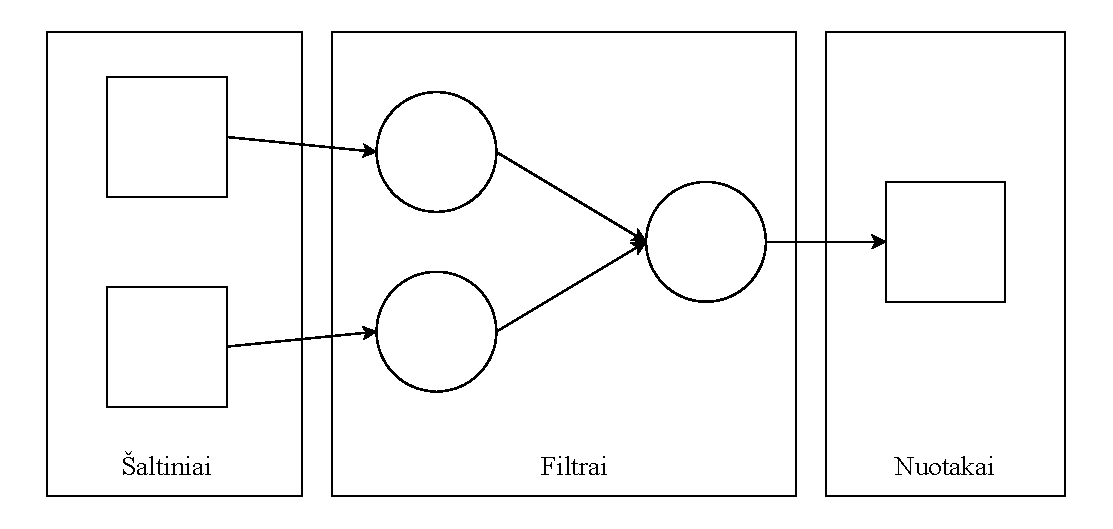
\includegraphics[width=15cm]{img/Srautinio apdorojimo sistema.pdf}
    \caption{Srautinio apdorojimo sistemos pavyzdys}
    \label{srautinio-apdorojimo-sistema}
\end{figure} 
Srautinio apdorojimo sistemos literatūroje yra vaizduojamos orientuotais grafikais (\ref{srautinio-apdorojimo-sistema} pav.). Srautinio apdorojimo sistemos skiriasi nuo reliacinių modelio šiais aspektais \cite{babcock2002models}: 
\begin{itemize}
    \item Duomenys į sistemą patenka tinklu, o ne iš fizinių talpyklų.
    \item Duomenų patekimo tvarka negali būti kontroliuojama.
    \item Duomenų kiekis yra neapibrėžtas.
    \item Duomenys apdoroti srautinio apdorojimo sistema yra pašalinami arba archyvuojami, t.y. juos pasiekti yra sunku. 
\end{itemize}
\subsubsection{Duomenų vykdymas}
Srautinio apdorojimo sistemų veikimui reikalingas srautinio apdorojimo variklis (angl. stream processing engine). Šie varikliai yra skirti srautinio apdorojimo sistemų vykdymui, dislokavimui, plečiamumo (angl. scaling) užtikrinimui ir gedimų tolerancijai (angl. fault–tolerance) \cite{zhao2017taxonomy}. Populiariųjų srautinio apdorojimo variklių pavyzdžiai: „Apache Storm“, „Apache Heron“, „Apache Spark“, „Apache Samza“ ir t.t \cite{roger2019comprehensive}. 
Duomenų vykdymas gali būti išskaidytas į tris elementus \cite{zhao2017taxonomy}: 
\begin{itemize}
    \item Planavimas (angl. scheduling) – duomenų apdorojimo užduočių planavimas daro įtaką bendram srautinio apdorojimo sistemos veikimui \cite{falt2011task}. Pavyzdžiui, „Apache Samza“ naudoja „Apache YARN“ resursų valdymo sistemą, kuri turi planavimo posistemę, kuri skirsto resursus \cite{noghabi2017samza} 
    \item Plečiamumas (angl. scalability) – apibrėžia daug apdorojimo branduolių turinčios sistemos gebėjimą apdoroti didėjanti kiekį užduočių ir galimybę didinti pačią sistemą, kad ji galėtų susidoroti su didėjančiu kiekiu duomenų \cite{bondi2000characteristics}. Srautinio apdorojimo varikliai turi užtikrinti srautinio apdorojimo sistemų plečiamumą \cite{stonebraker20058}.    
    \item Išskirstytas skaičiavimas (angl. Distributed computation) – tarpusavyje nesusiję skaičiavimo elementai turi naudotojui atrodyti kaip viena darni sistemą \cite{tanenbaum2007distributed}. Srautinio apdorojimo varikliai turi užtikrinti darbų paskirstymą ir skaičiavimo įrenginių koordinaciją, kad kuo daugiau duomenų būtų apdorojami vienu metu \cite{zhao2017taxonomy}.
\end{itemize}
Srautinio apdorojimo sistemos turi viena pagrindinį elementą – srauto procesorių (angl. stream processor), kuris apibrėžia sistemos elementus, aprašo kaip šie sistemos elementai sujungti ir pateikia nustatymus elementams \cite{zhao2017taxonomy}. Pavyzdžiui, „Apache Storm“ šis elementas vadinimas „topology“, kuris yra užrašomas Java kalba, naudojant „Apache Storm“ pateiktą biblioteką \cite{iqbal2015big}.
\subsubsection{Duomenų priėmimas}
Į srautinio apdorojimo sistemą duomenys patenka per šaltinius, kurie šiuos duomenis perduoda tolimesniems elementams. Dažniausiai duomenis perduodami į sistemą naudojant žinučių eiles (angl. message queues), nes jos turi buferi, kuris leidžia mažinti greičių skirtumus tarp duomenų gavimo ir duomenų apdorojimo ir žinučių eilių brokeriai gali išfiltruoti duomenis ir nukreipti juos į tinkamus šaltinius \cite{kamburugamuve2016survey}. Tačiau šaltiniai turi turėti galimybę rinkti išsaugotus duomenis ir priimti ateinančius naujus duomenis \cite{stonebraker20058}, todėl, nors ir šaltiniai dažniausiai skirti priimti srautinius duomenis, jie turi taip pat gebėti naudoti duomenis iš talpyklų \cite{zhao2017taxonomy}. 

\subsection{Srautinio apdorojimo sistemų matavimas}
Svarbiausias srautinio apdorojimo sistemų reikalavimas – duomenų apdorojimas ir rezultatų grąžinimas negali turėti atsilikimo – didelių apimčių srautiniai duomenys turi būti apdorojami taip pat greitai kaip jie ateiną \cite{stonebraker20058}. 

\subsubsection{Srautinio apdorojimo sistemų metrikos}
Pagrindinės kitų autorių naudojamos metrikos:
\begin{itemize}
    \item Pralaidumas (angl. Throughput) – per tam tikrą laiko tarpą apdorojamų įvykių kiekis.
    \item Vėlinimas (angl. Latency) – laiko intervalas nuo apdorojimo arba įvykio pradžios iki apdorojimo pabaigos.
\end{itemize}
Vėlinimas ir pralaidumas dažniausiai nepriklauso vienas nuo kito – sistemos, apdorojančios srautus mikro–paketais, turi didesnį pralaidumą, tačiau atsiranda papildomas vėlinimas, kol laukiama duomenų paketo apdorojimo pradžios \cite{Karimov2018BenchmarkingDS}. \par

\cite{stonebraker20058} straipsnyje minima, jog srautinio apdorojimo sistemos naudotojas turi išbandyti savo sistemą su tiksliniu darbo krūviu ir išmatuoti jos pralaidumą ir vėlinimą prieš naudodamas ją realiomis sąlygomis. \cite{Karimov2018BenchmarkingDS} lygina srautinio apdorojimo variklius ir matavimui naudoja vėlinimą, kurį išskaido į įvykio vėlinimą (angl. event–time latency) – laiko intervalas nuo įvykio laiko iki rezultato gavimo iš srautinio apdorojimo sistemos ir apdorojimo vėlinimą (angl. processing–time latency) – laiko intervalas nuo duomens patekimo į srautinio apdorojimo sistemą iki rezultato grąžinimo. Autoriai atlieka šį skaidymą, nes sistemų vertinime dažnai ignoruojamas įvykio laikas ir rezultatuose gaunamas daug mažesnis vėlinimas, nei tikras. Taip pat autoriai išskiria darnų pralaidumą (angl. sustainable throughput) – didžiausia apkrova įvykių, kurią sistema gali apdoroti be pastoviai augančio įvykio vėlinimo, todėl savo eksperimentuose autoriai užtikrina, kad duomenų generavimo greitis atitiktų sistemos darnų pralaidumą. Kad sužinoti darnų pralaidumą sistemos autoriai pradžioje leidžia labai didelį srautą duomenų ir mažina jį kol sistemos apdorojimas susivienodina su generavimo greičiais. Visus vėlinimo rezultatus autoriai pateikia maksimalaus pralaidumo apdorojimo ir 90\% pralaidumo apdorojimo vidurkiais, minimumais, maksimumais ir kvantiliais (90, 95, 99). \cite{hirzel2014catalog} autoriai nagrinėja srautiniam apdorojimui galimas optimizacijas ir matavimui naudoja normalizuotą pralaidumą (naudojamas vienetas kaip vidurkis), kadangi tai leidžia lengviau palyginti santykinę greitaveiką. Taip pat, \cite{hirzel2014catalog} pastebi, nors ir yra daug metrikų, kuriomis galima matuoti optimizacijos efektus: pralaidumas, vėlinimas, paslaugos kokybė (angl. quality of service), energijos ir tinklo panaudojimas, tačiau dažniausiai pagerinus pralaidumą pagerėja ir visos kitos metrikos. \cite{Qian2016Benchmarking} srautinių apdorojimo sistemų matavimui naudoja pralaidumą (skaičiuojama baitais per sekundę) ir vėlinimą, kaip vidurkį nuo duomens patekimo į sistemą iki apdorojimo pabaigos. Taip pat, kadangi autoriai lyginą srautinio apdorojimo variklius, jie įveda metriką gedimų toleravimo (angl. fault tolerance) matavimui – išjungiamas tam tikras kiekis elementų ir matuojamas pralaidumas ir vėlinimas. \cite{zhang2020heron} palyginimui naudoja sistemos įvykdymo vėlinimą (angl. system completion latency), kuris rodo vidutinį laiko tarpą per kurį duomuo nukeliauja nuo šaltinio iki sistemos galutinio taško. Autoriai skaičiavo vidutinį laiką 5 sekundžių intervalais. Taip pat autoriai matavimui naudoja kiekvienos instancijos (angl. instance) CPU apkrovą, kiekvieno darbinio mazgo (angl. worker node) CPU apkrovą ir apkrovą tarp instancijų/mazgų, kadangi \cite{zhang2020heron} užduotis – patobulinti esamą planavimo posistemę. \cite{dhalion} matavimui naudoja pralaidumą per minutę. \cite{vaquero2018autotuning} tyria labai panašią problemą – srautinių apdorojimo sistemų balansavimą taikant skatinamąjį mokymą ir matavimui naudoja vėlinimo 99 kvantilį. \cite{Chintapalli2016Benchmarking} srautinio apdorojimo variklių vertinimo tyrimui naudoja vėlinimą.

\begin{table}[H]
    \centering
    \caption{Metrikos naudojamos tiriant srautinio apdorojimo sistemų greitaveiką}
    \begin{tabular}{|l|l|l|}
    \hline
    Šaltinis                 & Vėlinimas                        & Pralaidumas                    \\ \hline
    \cite{stonebraker20058}  & Taip                             & Taip                           \\ \hline
    \cite{Karimov2018BenchmarkingDS} & Taip                     & Taip                           \\ \hline
    \cite{hirzel2014catalog} & Ne                               & Taip                           \\ \hline
    \cite{Qian2016Benchmarking} & Taip                          & Taip                           \\ \hline
    \cite{zhang2020heron}    & Taip                             & Ne                             \\ \hline
    \cite{dhalion}           & Ne                               & Taip                           \\ \hline
    \cite{vaquero2018autotuning} & Taip                         & Ne                             \\ \hline
    \cite{Chintapalli2016Benchmarking} & Taip                   & Ne                             \\ \hline
    \end{tabular}
\label{metrikos}
\end{table}

Pagal literatūros analizę (\ref{metrikos} len.) matome, kad dauguma autorių renkasi vertinti tik pagal vieną metriką ir dažniau matavimui naudojamas vėlinimas. Taip pat \cite{vaquero2018autotuning}, naudojantis skatinamąjį mokymą, matavimui naudoja vėlinimą ir \cite{Chintapalli2016Benchmarking} straipsnis, kuris siūlo srautinio apdorojimo sistemų vertinimo sprendimą, naudoja vėlinimą. Todėl magistro darbe matavimui bus naudojamas vėlinimas.   

\subsubsection{Srautinio apdorojimo sistemos pobūdis}

Srautinio apdorojimo sistemos gali turėti skirtingą elementų išsidėstymą ir nuo to priklausys jų greitaveiką. \cite{Karimov2018BenchmarkingDS} matavimui naudoja du filtrus – agregavimo, kuris skaičiuoja visus pirkimus ir jungimo (angl. join), kuris skaičiuoja duomenis pagal tam tikrą bendrą rodiklį iš abiejų duomenų srautų. \cite{Qian2016Benchmarking} srautinio apdorojimo variklių palyginimui naudoja septynis skirtingus uždavinius. Vienas iš jų yra WordCount uždavinys, kuris yra plačiai priimtas kaip didelių duomenų apdorojimo sistemos matavimo standartas \cite{huang2010hibench}. Šis uždavinys susidaro iš dviejų filtrų: pirmas išskaido teksto eilutę į žodžius, o antras agreguoja kiekvieno žodžio bendrą skaitiklį ir atnaujina bendrą žodžių panaudojimo dažnio rezultatą, kuriame raktas – žodis, o reikšmė skaičius, kuris rodo kiek kartojosi šis žodis (\ref{wordcount} pav.). 
\begin{figure}[H]
    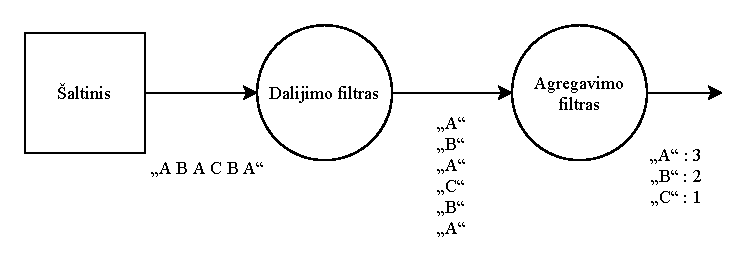
\includegraphics[width=15cm]{img/wordcount.pdf}
    \caption{WordCount sistemos pavyzdys}
    \label{wordcount}
\end{figure} 
\cite{zhang2020heron} matavimui naudoja WordCount sistemą, kuri yra paprastesnė, nei pavaizduota \ref{wordcount} paveikslėlyje, nes šaltinis generuoja ir siunčia tik po vieną žodį ir todėl yra tik agregavimo filtras. Taip pat autoriai  naudoja SentenceWordCount sistemą, kuri yra identiška \ref{wordcount} paveikslėlyje pavaizduotai sistemai. Bei autoriai sukūrė FileWordCount sistemą, kuri atlieka tą patį kaip ir SentenceWordCount, tačiau šaltinis negeneruoja žodžius, o skaito iš tekstinio dokumento ir taip pat naudoja egzistuojančią Yahoo srautinio apdorojimo vertinimą (angl. benchmarking) \cite{Chintapalli2016Benchmarking}. \cite{dhalion} autoriai naudoja WordCount eksperimentui. \cite{vaquero2018autotuning} eksperimentams naudoja Yahoo srautinio apdorojimo variklių vertinimą \cite{Chintapalli2016Benchmarking} ir taip pat atlieka bandymus su realiais daiktų interneto (angl. internet of things) įmonės duomenimis. \cite{Chintapalli2016Benchmarking} apibrėžia srautinio apdorojimo sistemą skirtingu srautinio apdorojimo variklių vertinimui. Pateikiama sistema analizuoja reklamas pagal kampaniją ir matomumą ir rezultatus deda į Redis duomenų bazę. Sistema sukurta taip, kad aprėptų visas srautinio apdorojimo sistemos savybes (\ref{yahoo} pav.).
\begin{figure}[H]
    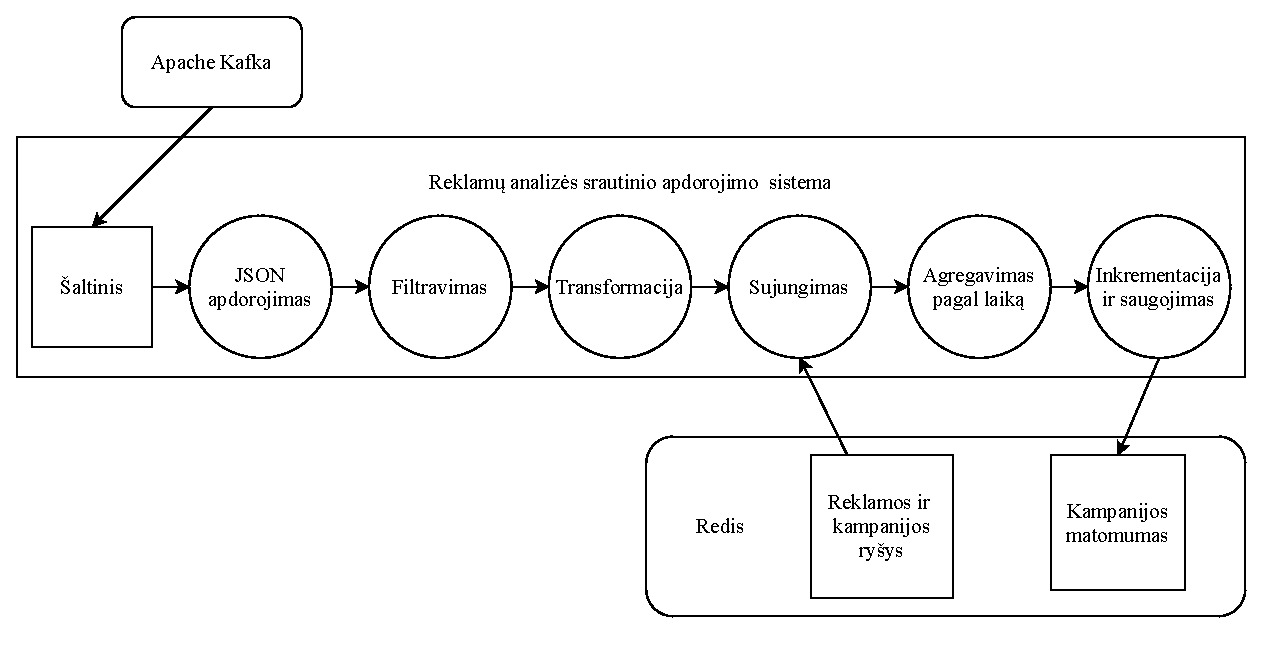
\includegraphics[width=15cm]{img/yahoo.pdf}
    \caption{Reklamų analizės sistema \cite{Chintapalli2016Benchmarking}}
    \label{yahoo}
\end{figure} 

Straipsniai (\cite{Qian2016Benchmarking, huang2010hibench, dhalion}) naudoja WordCount (\ref{wordcount} pav.), o \cite{Chintapalli2016Benchmarking, vaquero2018autotuning} naudoja Reklamų analizės srautinę apdorojimo sistemą (\ref{yahoo} pav.). Magistro darbe ketinama atlikti tyrimus su Reklamų analizės sistema, kadangi ši sistema sukurta srautinių apdorojimo variklių vertinimui ir su WordCount srautinio apdorojimo sistemą, kuri neturi pašalinių elementų sistemoje, kadangi Reklamų analizės sistema naudoja „Apache Kafka“, „Redis“ vertinimui.    

\subsubsection{Srautinio apdorojimo sistemų matavimo duomenys}

Vertinant sistemų greitaveiką reikia atsižvelgti ir į testavimui naudojamus duomenis. \cite{Karimov2018BenchmarkingDS} naudoja žaidimų kūrimo įmonės Rovio duomenis ir naudoja du duomenų srautus – pirkimo srautas, kuriame siunčiami kortežai (angl. tuples) sudaryti iš nupirktos valiutos kiekio, laiko ir naudotojo, kuris ją nupirko ir reklamų srautas, kuris siunčia valiutos reklamas tam tikru laiku. Šiame sprendime duomenis generuojami naudojant normalizuotą paskirstymą ant raktinio lauko. \cite{Qian2016Benchmarking} naudoja tekstinius duomenis iš AOL paieškos variklio ir apdoroja juos pagal pasirinktus uždavinius. \cite{zhang2020heron} matavimui naudoja šaltinių generuojamą tekstą, kadangi lyginamas tas pats srautinio apdorojimo variklis tik su patobulinta planavimo posisteme ir naudoja iš anksto sugeneruotą tekstą patalpintą į tekstinį dokumentą. \cite{Chintapalli2016Benchmarking} aprašo sistemą, kuri daro skirtingų srautinio apdorojimo variklių vertinimą. Šiam vertinimui naudojami duomenys simuliuojantys reklamas ir reklamų kampanijas. Autoriai naudoja savo duomenų generatorių. 
Magistro darbe ketinama naudoti \cite{Chintapalli2016Benchmarking} pateikiamą Reklamos analizės sistemos duomenų generatorių, o WordCount srautinės apdorojimo sistemos tyrimui ketinama naudoti WordCount šaltinio generuojamus duomenis.

\subsection{Srautinio apdorojimo sistemų derinimas}
Sistemų greitaveika yra tiesiogiai susijusi su konfigūravimo parametrais, kurie valdo tokius aspektus kaip: atminties valdymas, gijų skaičius, planavimas, resursų valdymas \cite{lu2019speedup}. Taip pat, neteisingi nustatymai turi nuostolingus efektus sistemos greitaveikai ir stabilumui \cite{herodotou2011starfish}. 

\cite{herodotou2020survey} išskiria 3 pagrindinius automatinio derinimo iššūkius:
\begin{enumerate}
    \item Didelė ir sudėtinga parametrų erdvė – „Apache Spark“ ir „Apache Storm“ turi virš 150 konfigūruojamų parametrų \cite{Bilal2017Towards, petridis2016spark}. Taip pat, nustatymų reikšmės, kurios tinka vienam uždaviniui, gali turėti neigiamos įtakos kitam \cite{herodotou2011starfish, Pooyan2016Uncertainty}.
    \item Sistemų mastas ir sudėtingumas – Sistemų administratoriai turi gebėti konfigūruoti didelius kiekius skaičiavimo mazgų, kurie gali turėti skirtingus CPU, atminties, tinklo tipus \cite{herodotou2020survey}.
    \item Pradinių duomenų statistikos trūkumas – įvedimo duomenys srautinėse apdorojimo sistemose yra realus srautai, kurie stipriai varijuoja savo apimtimi \cite{Dayarathna2018Recent}.
\end{enumerate}  

\cite{Trotter2017Into} nagrinėjantis tinkamos konfigūracijos radimą naudojant genetinius algoritmus „Apache Storm“ srautinio apdorojimo sistemoms nustatė, jog lygiagretumo laipsnis labiausiai daro įtaką srautinio apdorojimo sistemų greitaveikai. „Apache Heron“ srautinio apdorojimo variklis, kuris yra „Apache Storm“ su patobulinimais \cite{twitterHeron}, pateikia naują būdą kontroliuoti srautą – priešslėgis (angl. backpressure), kuris leidžia filtrui sulėtinti prieš jį einantį elementą, kas leidžia sumažinti vėlinimą ir taip pat gali būti naudojamas kaip greitaveikos praradimo indikatorius \cite{bansal2018trevor}.
Taip pat \cite{bansal2018trevor} nagrinėja „Apache Heron“ automatinį konfigūravimą naudojant iš anksto aprašytas taisykles. 

\section{Mašininis mokymasis}

\subsection{Mašininis mokymasis srautinio apdorojimo sistemų derinimui}

\cite{herodotou2020survey} aprašo skirtingus sprendimus automatiniam konfigūravimui ir išskiria šiuos mašininio mokymosi privalumus:
\begin{itemize}
    \item Nebūtina suprasti sistemos, užduočių ir duomenų, kadangi naudojamas juodos dėžės (angl. black–box) principas.
    \item Mašininio mokymosi modelis pats save tobulina, ir yra vis tikslesnis kuo daugiau gauna duomenų. 
\end{itemize}
Šio straipsnio autoriai išskiria mašininio mokymosi iššūkius: 
\begin{itemize}
    \item Parametrų parinkimas – kadangi konfigūruojamų parametrų kiekis yra didelis \cite{Bilal2017Towards, petridis2016spark} ne visi iš jų vienodai daro įtaką greitaveikai, todėl pirma verta išsirinkti aktualiausius parametrus resursų valdymo, užduočių planavimo ir duomenų valdymo užduotims. Tam dažnai naudojama eksperto pagalba \cite{wang2016novel}, gidai arba eksperimentavimas. Tačiau galima naudoti mašininio mokymosi algoritmą koreliacijos nustatymui tarp parametrų ir greitaveikos \cite{vaquero2018autotuning, yang2012statistics}
    \item Mašininio mokymosi modelio pasirinkimas – kadangi yra nemažai skirtingų mašininio mokymosi metodų kurie tinka derinimo uždaviniui.
\end{itemize} 
Taip pat autoriai pateikia paketinio ir srautinio apdorojimo derinimą naudojant mašininį mokymąsi straipsnius (\ref{ml-in-stream} lentelėje pateikiami tik išrinkti srautinio apdorojimo pavyzdžiai).

\begin{table}[H]
    \centering
    \caption{Srautinių sistemų derinimo naudojant mašininį mokymąsi pavyzdžiai \cite{herodotou2020survey}}
    \begin{tabular}{|l|p{0.40\textwidth}|p{0.20\textwidth}|}
    \hline
    Šaltinis                                        & Įvesties savybės                                                                    & Mašininio mokymosi metodai                 \\ \hline
    Zacheilas et al. \cite{zacheilas2015elastic}    & Rinkinys kelių konfigūracijos parametrų                                             & Gaussian Processes                         \\ \hline
    Li et al. \cite{li2016performance}              & Atminties dydžiai ir branduolių ir gijų kiekis skirtingose stadijose                & Support Vector Regression                  \\ \hline
    Trotter et al. \cite{Trotter2017Into}           & Darbinių procesų kiekis, vykdytojų kiekis                                           & Genetic Algorithm, Bayesian Optimization   \\ \hline
    Trotter et al. \cite{trotter2019forecasting}    & Vykdytojai, šaltinių ir filtrų lygiagretumas, acker lygiagretumas                   & Genetic Algorithm, Support Vector Machines \\ \hline
    OrientStream \cite{wang2017automating}          & Įvairios duomenų, plano, filtrų ir klasterio lygio savybės                          & Ensemble/ Incremental ML                    \\ \hline
    Vaquero et al. \cite{vaquero2018autotuning}     & Parametrai ir metrikos parinkti faktorinės analizės (angl. factor analysis) pagalba & Reinforcement Learning                     \\ \hline
    \end{tabular}
    \label{ml-in-stream}
\end{table}

\subsection{Skatinamasis mokymasis srautiniam apdorojimui}

\cite{vaquero2018autotuning} nagrinėja srautinių sistemų derinimą naudojant skatinamąjį mokymąsi. Autoriai pradžioje pasirenka Lasso path analysis algoritmą, kurio pagalba atlieka parametrų atranka, kad išrinktų svarbiausius parametrus pasirinktos metrikos valdymui. Konfigūracijos valdymui pasirinktas modifikuotas REINFORCE algoritmas. Atliktas eksperimentas su „Apache Spark“, kuris rodo 60–70\% sumažintą vėlinimą.

\cite{ni2019generalizable} nagrinėja resursų valdymo problemą srautinio apdorojimo sistemose ir siūlo sprendimą naudojanti skatinamąjį mokymą, kuris daro optimizacijas pagal srautinės apdorojimo sistemos grafus. Eksperimentas atliekamas naudojant REINFORCE \cite{williams1992simple} algoritmą su Adam optimizacijos funkcija \cite{kingma2014adam} ir atliekamas eksperimentas naudojant tyrimui parašytą srautinio apdorojimo variklį ir sistemas. 

\cite{Li2018Model} nagrinėja planavimo problemos (apkrovos paskirstymas darbiniams elementams) sprendimą naudojant skatinamąjį mokymąsi. Autoriai siūlo naudoti Actor−Critic {lillicrap2015continuous} metodą naudojant Deep Q Learning  \cite{mnih2015human} tinklą kaip Actor ir bet kokį gilųjį neuroninį tinklą kaip Critic. Autorių rezultatai rodo 45\% greitaveikos padidėjimą lyginant su integruota „Apache Storm“ planavimo posisteme. 

\cite{Russo2019Reinforcement} nagrinėja srautinių sistemų dislokavimą naudojant skatinamąjį mokymą. Sprendžiama problema dislokavimo valdymo su skirtingais skaičiavimo mazgų tipais. Naudojamas Q Learning algoritmas su įvairioms modifikacijom (kombinuojama su tiksliais modeliais). Autoriai matuoja dislokavimo tikslumą ir konvergavimo greitį. 

\begin{table}[H]
    \centering
    \caption{Skatinamojo mokymosi naudojimas}
    \begin{tabular}{|l|l|}
    \hline
    Šaltinis                         & Skatinamojo mokymosi algoritmas    \\ \hline
    \cite{vaquero2018autotuning}     & Adaptuotas REINFORCE \cite{williams1992simple}        \\ \hline
    \cite{ni2019generalizable}       & REINFORCE \cite{williams1992simple}  su Adam optimizacijos funkcija \cite{kingma2014adam}     \\ \hline
    \cite{Li2018Model}               & Deep Q Learning \cite{mnih2015human} ir Actor−Critic \cite{lillicrap2015continuous} \\ \hline
    \cite{Russo2019Reinforcement}    & Q–learning \cite{mnih2015human} su papildomomis funkcijomis \\ \hline
    \end{tabular}
    \label{ml-in-stream}
\end{table}


\sectionnonum{Išvados}

\begin{enumerate}
    \item Išnagrinėjus literatūrą nustatyta, kad:
        \begin{itemize}
            \item matavimui tinka Reklamos analizės sistema, kadangi ji yra sukurta ir naudojama kaip vertinimo standartas srautinio apdorojimo varikliams, ir WordCount sistema, kadangi ji neturi pašalinių elementų, kurie gali sukurti trukdžius ir yra naudojama kitų autorių moksliniuose darbuose.
            \item duomenų generavimui tinka naudoti \cite{Chintapalli2016Benchmarking} duomenų generatorių Reklamos analizės sistemos bandymui, kuris yra pateikiamas kartu su srautinio apdorojimo variklių vertinimu ir WordCount šaltinio duomenų generatorių WordCount eksperimentams.
            \item sprendimų greitaveikos vertinimui tinka naudoti vėlinimą, kadangi \cite{Chintapalli2016Benchmarking} naudoja vėlinimą srautinio apdorojimo variklių vertinimui bei kiti autoriai naudoja vėlinimą siūlomų sprendimų greitaveikos įrodymui.  
        \end{itemize}
    \item Deep Q Learning ir Actor–Critic algoritmai yra tinkami skatinamojo mokymosi algoritmai srautinio apdorojimo sistemų derinimui, atsižvelgus į jų naujumą ir tinkamumą nagrinėti pastovaus valdymo uždavinius \cite{Silver2014Deterministic}. Taip pat atsižvelgus į \cite{vaquero2018autotuning, herodotou2020survey} rezultatus yra rekomenduojama atlikti bandymus su sumažinta konfigūruojamų elementų aibe naudojant parametrų parinkimą, atlikti bandymus su nekeista elementų aibe ir palyginti rezultatus.
\end{enumerate}

\printbibliography[heading=bibintoc] 

\end{document}
